\documentclass{article}
\usepackage{graphicx}
\usepackage[T2A]{fontenc}
\usepackage[a4paper, margin=25mm, left=20mm, top=25mm, right=20mm, bottom=20mm, head=20mm, nofoot] {geometry}
\usepackage[utf8]{inputenc}
\usepackage{array}
\usepackage[russian]{babel}
\usepackage{float}


\title{Дизайн документ}
\author{Андриянов Арсений, Александрова Ксения, Левицкая Алиса, \\ Печалинова Богдана, Соболев Григорий}


\date{Ноябрь 2024}

\begin{document}
	
	\maketitle
	
	\tableofcontents
	
	\newpage
	\section{Введение}
	Дальнейшее содержание этого документа организовано по разделам, в которых приводится следующая информация:
	\begin{itemize}
		\item Раздел 2. Концепция. Данный раздел содержит основные сведения об игре, включая общее описание, жанр, целевую аудиторию, предпосылки создания и основные особенности игры, а также информацию о платформах, на которых она будет доступна.
		\item Раздел 3. Функциональная спецификация. Этот раздел детально описывает функциональные аспекты игры, такие как принципы игрового процесса, физическая модель, характеристики персонажа, элементы игры, искусственный интеллект, многопользовательский режим, интерфейс пользователя, графика и видео, звуки и музыка, а также описание уровней.
		\item Раздел 4. Контакты. Данный раздел содержит контактную информацию для связи с разработчиками или другими заинтересованными лицами.
	\end{itemize}
	
	\newpage
	\section{Концепция}
	
	\subsection{Введение}
	Игра сочетает элементы \textit{хоррора, приключений, ролевой игры и мистического сюрреализма с головоломками и пиксельной графикой}. Она предназначена для аудитории от \textbf{14 лет и старше}. Игроки погружаются в мрачный и серый мир повседневной жизни, где реальность переплетается с мистикой, и каждое решение приводит к новым последствиям. Проект отличается напряженной атмосферой, нелинейным сюжетом, стратегическими элементами и глубоким нарративом, затрагивающим социальные и психологические проблемы, что делает его привлекательным для фанатов инди-разработок и атмосферных хорроров.
	
	\subsection{Жанр и аудитория}    
	Жанр игры можно определить как \textit{хоррор-приключенческий} с элементами ролевой игры, мистического сюрреализма и пиксельной графикой с головоломками. Игрокам предстоит погрузиться в мрачный и серый мир повседневной жизни обычного человека рабочего класса, где они столкнутся с различными мистическими загадками и кошмарами, отражающими истинные страхи людей в современного мире. \\  
	
	Игра ориентирована на взрослую аудиторию, в основном от \textbf{14 
		лет и старше}, что обусловлено наличием напряженной атмосферы и хоррор-сцен, а также сложных тем, которые могут не подойти более юной аудитории. Кроме того, игра привлекает людей, интересующихся инди-разработками и атмосферными, завлекательными нарративами, а также теми, кто хочет исследовать социальные и психологические проблемы, волнующие почти каждого человека на ежедневной основе. \\

	\subsection{Основные особенности игры}
	
	\textit{Ключевая особенность} игры состоит в том, что игрок вводится в игру не диалогами и записками, а посредством визуальных, звуковых и геймплейных деталей. Основная игровая задача -- передать атмосферу и эмоции главного героя через мрачные сочетания тонов, напряженные звуки и относительно высокую сложность игры. Также почувствовать ответственность за исход игры позволяет возможность игрока повлиять на развитие сюжета своими действиями.\\
	
	\textit{Длительность} прохождения зависит от игрока: от его адаптированности к подобному жанру и выбора концовки. Прохождение займет у игрока от 2 до 5 часов.\\

	\subsection{Описание игры} 
	
	\textit{The Twilight World} -- это увлекательная приключенческая игра, где игроки погружаются в новый мир, исследуя загадочные земли и решая разнообразные головоломки. Игра предлагает уникальный сюжет, насыщенный интересными персонажами и захватывающими квестами.\\
	
	Сюжет игры развернётся вокруг обычного человека, внезапно оказавшегося в мрачном, мистическом мире, где реальность искажена, а привычные места превратились в опасные лабиринты. Его главная цель -- выбраться живым и понять, \textit{что} привело его сюда.   
	Сначала главный герой начнёт замечать странные события: шепоты из пустых комнат, движущиеся тени и непонятные символы. По мере продвижения он найдет подсказки и артефакты, которые помогут понять природу происходящего, но для этого потребуется внимательность и логическое мышление. Ему также предстоит встречаться с таинственными сущностями, которые могут либо помочь, \textit{либо сбить с пути}. \\
	
	Сюжет будет нелинейным -- игроку придётся принимать решения, от которых зависят финал и разгадывания главной тайны. Игра создаст напряжённую атмосферу, где каждый шаг может привести как к спасению, так и к гибели, а загадки реального мира переплетаются с мистикой. \\
	

	\newpage
	\subsection{Предпосылки создания}
	
	Идея игры основывается на растущей популярности проектов, сочетающих психологический хоррор и элементы головоломки. Атмосферные инди-хорроры популярны в наши дни, как и игры с сильным визуальным стилем и глубоким сюжетом. Существование игр, совмещающих подобные жанры (например, "Yuppie Psycho", "Rusty Lake", "Amanda The Adventurer") демонстрирует, что игроки ищут в хорроре не только адреналин, но и глубокую историю с атмосферой, способной погрузить их в мир загадок, тревог и интриг. Данная игра предлагает уникальное сочетание: исследование мрачного, но знакомого мира, где реальность переплетается с мистикой, а каждое решение приводит к новым последствиям. \\
	
	\textit{Тенденции рынка:} сейчас растет популярность инди-игр с акцентом на хоррор стиль и атмосферу. Различные платформы (Steam, Epic Games) активно поддерживают проекты, которые выделяются своей эстетикой и идеей. Чёрно-белая палитра, минимализм и мистические элементы уже доказали свою успешность, привлекая как нишевых фанатов, так и широкую аудиторию. Кроме того, наличие нелинейного сюжета и элементов стратегии позволяет привлечь не только поклонников хорроров, но и игроков, ищущих интеллектуальные вызовы и разветвления в сюжете.
	
	\textit{Лицензирование и оригинальность:} весь игровой контент создаётся с упором на креативность, чтобы предложить уникальный продукт. Сюжет, персонажи и механики полностью авторские. \\
	
	Игры ужасов ценны своей способностью вызывать глубокий страх, который сложно испытать в реальной жизни, а эффект напряжения и последующего расслабления приносит игроку положительные эмоции. Наша игра построена на постоянном ощущении напряжения и дискомфорта, а не на банальных драках, что делает ее более осмысленной и эмоционально насыщенной. Это не просто аттракцион, а возможность для игрока испытать сложные чувства, исследуя мир, где мистика и реальность переплетаются. Проект имеет право на жизнь благодаря оригинальности концепции, сочетанию захватывающего геймплея с визуальным искусством и востребованности подобных игр на рынке.
	
	\subsection{Платформа}
	
	\begin{table}[h!]
		\centering
		\renewcommand{\arraystretch}{1.5}
		\setlength{\tabcolsep}{8pt}
		\begin{tabular}{|p{0.25\textwidth}|p{0.3\textwidth}|p{0.3\textwidth}|}
			\hline
			\multicolumn{3}{|c|}{\textbf{Для Windows}} \\ \hline
			\textbf{Требования} & \textbf{Минимальные} & \textbf{Рекомендуемые} \\ \hline
			\textit{Операционная система} & Windows 7 & Windows 10 \\ \hline
			\textit{Процессор} & Quad-core Intel \newline или AMD processor & Intel Core i5 \\ \hline
			\textit{ОЗУ} & 2 GB & 4 GB \\ \hline
			\textit{CD-ROM привод} & Нет & Нет \\ \hline
			\textit{Свободное место на HDD} & 4 GB & 4 GB \\ \hline
			\textit{Видеокарта} & NVIDIA GeForce 9800 GT \newline или AMD Radeon HD 4870 & NVIDIA GeForce GTX 750 Ti \newline или AMD Radeon R7 260X \\ \hline
			\textit{Звуковая карта} & Совместимая с DirectX 9.0c & Совместимая с DirectX 12 \\ \hline
			\textit{Управление} & Клавиатура и мышь & Клавиатура, мышь, геймпад \\ \hline
		\end{tabular}
		\caption{Системные требования для Windows}
		\label{tab:system-requirements1}
	\end{table}
	
	\begin{table}[h!]
		\centering
		\renewcommand{\arraystretch}{1.5}
		\setlength{\tabcolsep}{8pt}
		\begin{tabular}{|l|c|c|}
			\hline
			\multicolumn{3}{|c|}{\textbf{Для macOS}} \\ \hline
			\textbf{Требования} & \textbf{Минимальные} & \textbf{Рекомендуемые} \\ \hline
			\textit{Операционная система} & macOS X 10.8 & macOS 13.0 Ventura \\ \hline
			\textit{Процессор} &  Intel Core 2 Duo & Apple M1 \\ \hline
			\textit{ОЗУ} & 2 GB & 2 GB \\ \hline
			\textit{CD-ROM привод} & Нет & Нет \\ \hline
			\textit{Свободное место на HDD} & 4 GB & 4 GB \\ \hline
			\textit{Видеокарта} & Intel(R) HD Graphics 520 & Dedicated GPU supporting OpenGL \\ \hline
			\textit{Звуковая карта} & Встроенная & Встроенная \\ \hline
			\textit{Управление} & Клавиатура и мышь & Клавиатура, мышь, геймпад \\ \hline
		\end{tabular}
		\caption{Системные требования для macOS}
		\label{tab:system-requirements2}
	\end{table}
	
	\newpage
	\section{Функциональная спецификация}
	
	\subsection{Принципы игры}
	
	\subsubsection{Суть игрового процесса}
	 
	 Игровой процесс нашей игры предлагает глубокое погружение в мрачный и загадочный мир, где каждая деталь имеет значение, а каждое действие влияет на дальнейшее развитие сюжета. Основной акцент сделан на исследовании напряженной атмосферы и задачах, требующих внимательности и логического мышления, которые держат игрока в постоянном напряжении и заставляют задумываться над каждым шагом. \\
	 
	 \textbf{Основные эелементы геймплея:}
	 
	 \textit{Исследование.} Игрок перемещается по запутанным локациям, полным загадок, потайных ходов и интерактивных объектов. Мир наполнен скрытыми символами, записками и странными предметами, которые раскрывают детали сюжета. Каждая локация предлагает новые интерактивные элементы, будь то тайный замок, головоломка или необычный механизм, который необходимо активировать. Игроку предстоит внимательно осматривать окружение, чтобы находить ключи, подсказки и предметы для выживания.
	 
	 \textit{Головоломки.} Каждая локация предполагает логические задачи, которые тесно связаны с сюжетом. Игроку предстоит разгадывать шифры и символы, связанные с мистической историей, искать спрятанные механизмы и активировать их в правильной последовательности, собирать фрагменты информации для решения глобальных загадок, которые раскрывают ключевые аспекты мира игры.
	 
	 \textit{Элементы выживания и стратегия.}  Игроку придется управлять ограниченными ресурсами, включая здоровье,  редкие предметы и уникальные инструменты, такие как шприц с зеленым ядом. Принятие решений играет ключевую роль, игрок будет задаваться вопросом: "Использовать найденный предмет сейчас или сохранить его для более опасного момента?". Некоторые выборы будут влиять на развитие сюжета, изменение взаимоотношений с персонажами и конечного исхода игры.
	 
	 \textit{Сюжетное погружение.} История раскрывается через взаимодействие с миром, встречи с NPC и изменения в окружении. Игрок будет исследовать как реальные, так и мистические элементы, постепенно узнавая больше о природе происходящего. Сюжет развивается нелинейно, предлагая разные концовки в зависимости от решений игрока. \\
	 
	 Игра предложит игроку уникальный опыт: не только хоррор для андреналина, но и интеллектуальное, эмоционально насыщенное приключение, где страх и тайна создают незабываемую атмосферу. Игрок будет в постоянном напряжении и испытывать чувство неизвестности, а также удовольствия от постепенного раскрытия сложной и мистической истории. \\
	
	\subsubsection{Ход игры и сюжет}
		
	В этом хорроре игрока ожидает уникальный опыт, сочетающий напряженную атмосферу, глубокую интригу и необычную динамику взаимодействия с миром. Геймплей строится на исследовании, принятии решений и постоянной борьбе с неизвестным, заставляя задуматься о своей роли в происходящем. История медленно раскрывает связь главного героя с потусторонними событиями, держит в состоянии постоянного саспенса и предлагает искать ответы на непростые вопросы.
	
	Сеанс игры начинается с минималистичного меню. На экране – приглушенные тени, едва заметное мерцание и тихий шепот, создающий ощущение тревоги. После выбора "новая игра" начинается вступительная сцена, погружающая в историю. \\
	
	\textbf{Ход игры:}
	
	\textit{Игра открывается с видения:} в таинственном, искаженном мире раздаются голоса. Неопределенные фигуры, похожие на тени с размытыми очертаниями лиц, спорят о судьбе человека. Одни видят в нем ключ для восстановления порядка, другие – угрозу. Их спор прерывается яркой вспышкой, и игрок оказывается в обыденном офисе. За рабочим столом  просыпается главный герой, окруженный привычной суетой рабочего дня, но с самого начала что-то кажется не так.
	
	\begin{figure}[h]
		\centering
		\begin{minipage}{0.45\textwidth}
			\centering
			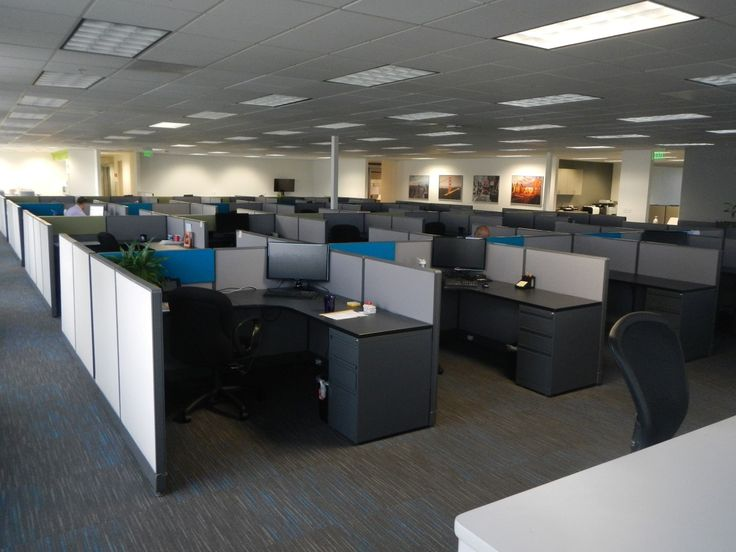
\includegraphics[width=\textwidth]{images/officeReference.jpg}
			\caption{Референс офиса}
			\label{fig:office}
		\end{minipage}
		\hfill
		\begin{minipage}{0.45\textwidth}
			\centering
			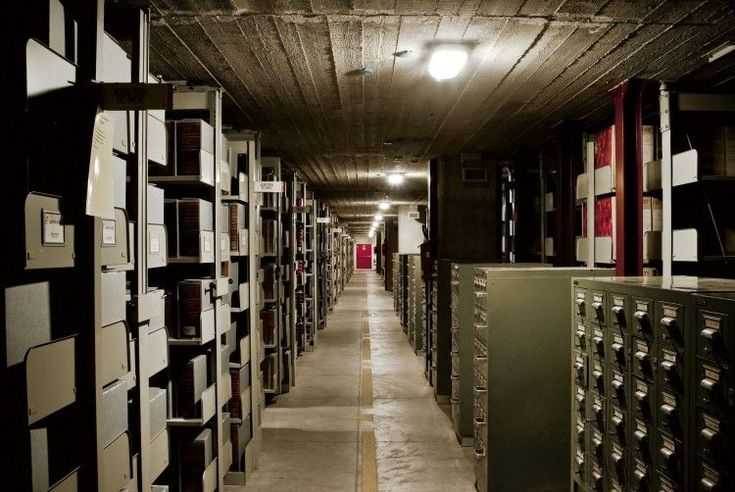
\includegraphics[width=\textwidth]{images/archive1.jpg}
			\caption{Референс архива}
			\label{fig:archive}
		\end{minipage}
	\end{figure}
	
	Игроку предоставляется возможность \textit{исследовать} офис. Задачи просты: взаимодействовать с предметами, читать записки, исследовать детали окружающего мира. Однако реальность постепенно становится всё более странной: часы идут в обратном направлении и растекаются, из мониторов доносится шепот, а лампы выключаются. Среди странностей – письмо, в котором намекается на скрытый архив. Игроку предстоит разгадать, как добраться до этой загадочной комнаты.
	
	\begin{figure}[H]
		\centering
		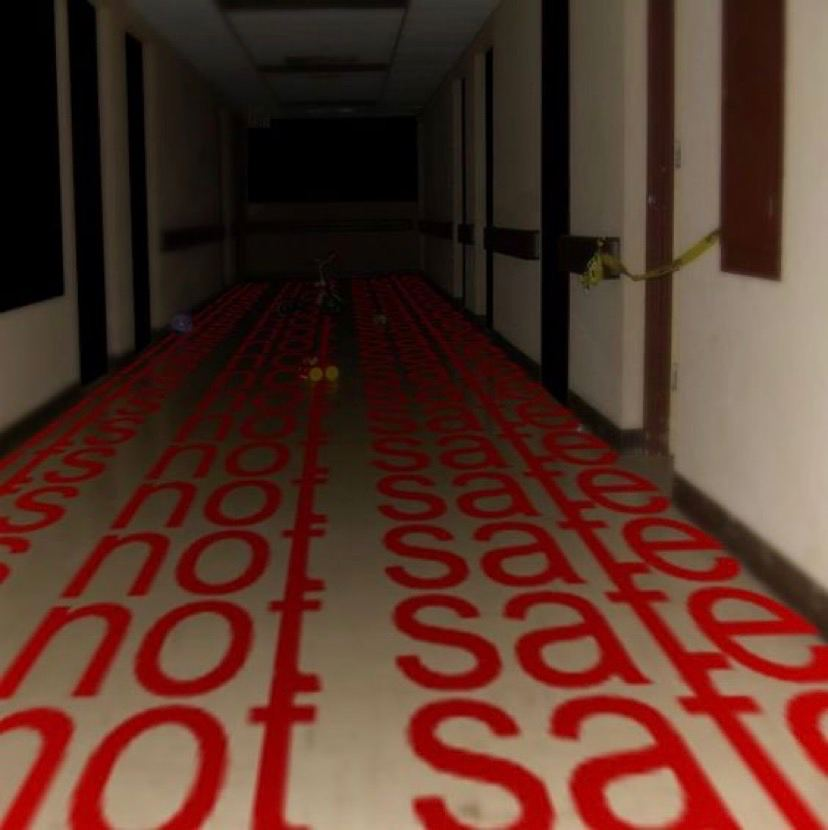
\includegraphics[width=0.4\textwidth]{images/pathtoarchive.jpg}
		\caption{Референс пути к архиву}
		\label{fig:path}
	\end{figure}
	
	\newpage
	 \textit{Переход в потусторонний мир} происходит неожиданно. В архиве герой находит странный артефакт. Прикосновение вызывает вспышку, после которой мир меняется. Потусторонняя реальность полна искажений: тени становятся укрытием, свет – опасностью, а правила подчиняются неведомым силам. Здесь игроку придется адаптироваться к новым условиям и исследовать, как же связан герой с этим миром. На протяжении игры герой будет разгадывать загадки, исследовать переходы между мирами и взаимодействовать с таинственными предметами, чтобы понять причины хаоса и его влияние на обе реальности.
	 
	 \begin{figure}[h]
	 	\centering
	 	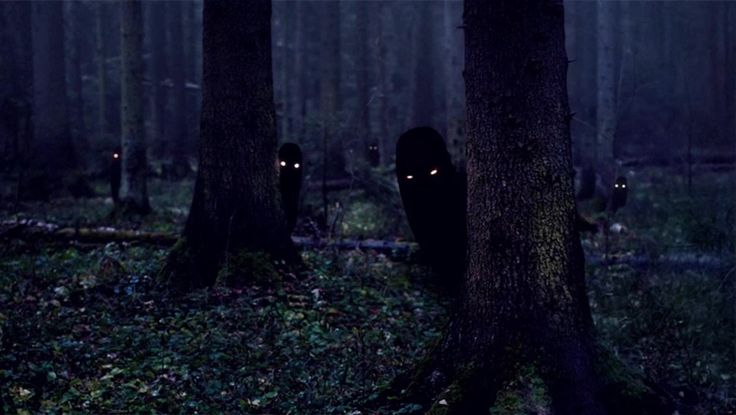
\includegraphics[width=0.45\textwidth]{images/otherworld.jpg}
	 	\caption{Референс потустороннего мира}
	 	\label{fig:otherworld}
	 \end{figure}
	 
	В процессе герой сталкивается с \textit{таинственными существами} – тенями, чьи маски отображают скрытые эмоции, и монстрами, собранными из фрагментов реальности. Одни из них предлагают помощь, другие ставят перед ним задачи или загадки. Но всегда остается вопрос: точны ли их намерения?
	
	\begin{figure}[h]
		\centering
		\begin{minipage}{0.45\textwidth}
			\centering
			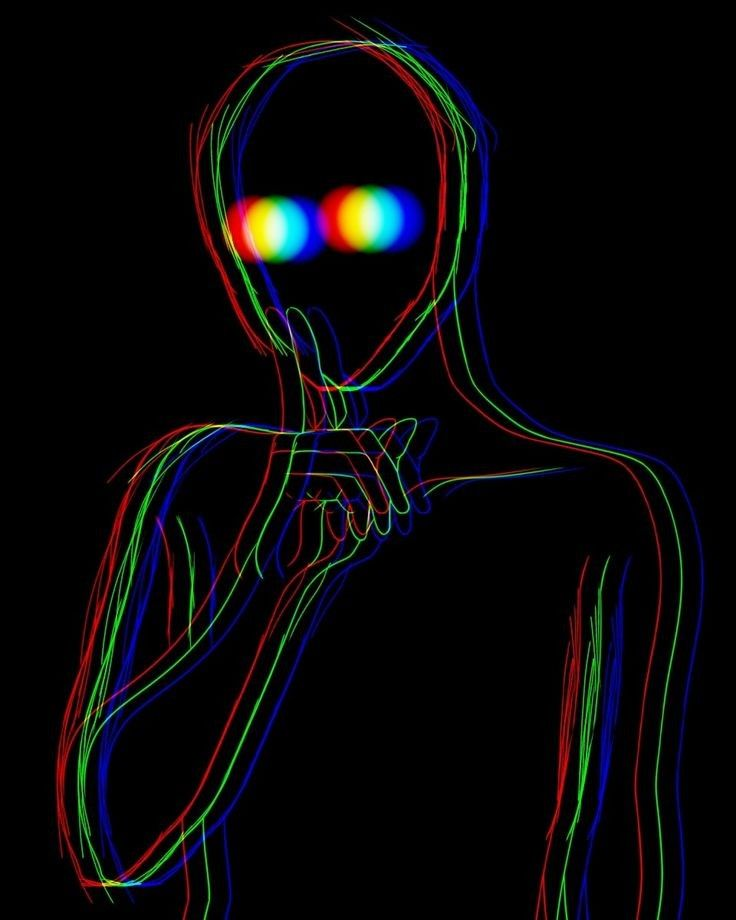
\includegraphics[width=\textwidth]{images/entity3.jpg}
			\caption{Референс таинственной сущности}
			\label{fig:entity1}
		\end{minipage}
		\hfill
		\begin{minipage}{0.4\textwidth}
			\centering
			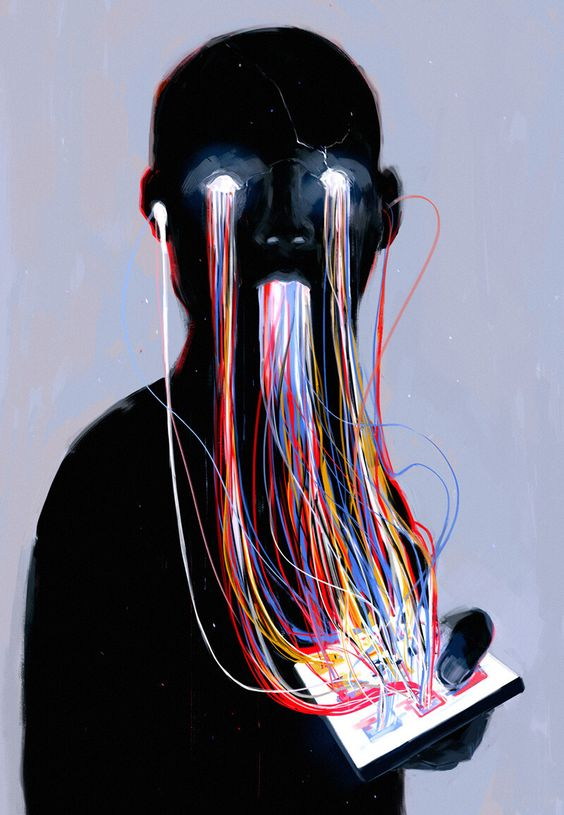
\includegraphics[width=\textwidth]{images/entity4.jpg}
			\caption{Референс таинственной сущности}
			\label{fig:entity2}
		\end{minipage}
	\end{figure}
	
	
	Сюжет разворачивается через загадки, диалоги и открытия. Игрок будет переходить между мирами, влияя на их состояние своими решениями. Офис и потусторонний мир становятся зеркалами, где действия героя оставляют след.
	
	\textit{Финал игры} держит в тайне истинные намерения всех сторон. Выборы игрока формируют концовку, но оставляют место для сомнений: правильно ли поступил герой? Почему коллеги избегают его взгляда? Что скрывают существа с другой стороны, называя его ключом? Кто из окружающих действительно хочет помочь, а кто скрывает истинные намерения? \\
	
	\newpage
	\textbf{Лор и история вселенной:}
	
	Потусторонний мир – это результат неудачных экспериментов по созданию порталов между человеческим сознанием и его тенью. Учёные хотели создать пространство чистого разума, но открыли двери в измерение, где человеческие страхи, желания и эмоции обретают форму.
	
	Этот мир наполнен существами, рожденными из подавленных эмоций. Одни стремятся уничтожить границы между реальностями, другие пытаются сохранить баланс. Герой оказывается втянут в эту историю, но вопрос остается открытым: случайно ли?
	
	Судьба мира зависит от игрока, но правда о герое может оказаться гораздо сложнее. Кто он в этой истории: спаситель, разрушитель или пешка в чужой игре?

	\subsection{Физическая модель}
    
        \newpage
	\subsection{Персонаж игрока}
    Главный герой — обычный офисный работник, который ведет рутинную жизнь, погруженный в повседневные заботы и обязанности. Однако его привычный мир резко меняется, когда он оказывается в мрачном и искаженном пространстве, полном загадок и опасностей. Внешне он ничем не примечателен: скромная офисная одежда и обыденная внешность делают его похожим на тысячи других людей. Тем не менее, за этой непримечательной оболочкой скрывается умение анализировать ситуацию и находить нестандартные решения.

    В новом мире герой сталкивается с множеством испытаний, требующих от него смелости и решительности. Он понимает, что для того чтобы выжить и найти путь обратно, ему нужно использовать свои способности для решения головоломок и разгадки тайн, окружающих его. Каждый шаг требует внимания и осторожности, а каждое открытие приближает его к пониманию причин своего появления в этом странном месте.

    Основная цель героя — выбраться из этого мрачного мира и понять причины своего появления здесь. Каждый его шаг и каждое решение могут существенно повлиять на развитие сюжета и финал истории. В процессе путешествия он будет сталкиваться с различными выборами, которые могут привести к неожиданным последствиям. 

	\begin{figure}[h]
		\centering
		
\includegraphics[width=0.45\textwidth]{images/main.jpg}
		\caption{Референс персонажа игрока}
		\label{fig:otherworld}
	\end{figure}
        
	\newpage
	\subsection{Элементы игры}
	
	\subsection{«Искусственный интеллект»}
	
	\subsection{Интерфейс пользователя}
	
	\subsubsection{Блок-схема}
	
	\subsubsection{Функциональное описание и управление}
	
	\subsubsection{Объекты интерфейса пользователя}
	
	\subsection{Графика и видео}
	
	\subsubsection{Общее описание}
	
	\subsubsection{Двумерная графика и анимация}
	
	\subsubsection{Трехмерная графика и анимация}
	
	\subsubsection{Анимационные вставки}
	
	\subsection{Звуки и музыка}
	
	\subsubsection{Общее описание}
	
	\subsubsection{Звук и звуковые эффекты}
	
	\subsubsection{Музыка}
	
	\subsection{Описание уровней}
	
	\subsubsection{Общее описание дизайна уровней}
	
	\subsubsection{Диаграмма взаимного расположения уровней}
	
	\subsubsection{График введения новых объектов}
	
	\newpage
	\section{Контакты}
	
	\newpage
	
\end{document}
